% !TeX root = ../UrrutiaAnguiano_CandidaturaDefensa.tex
% !TeX spellcheck = es_MX 


{\setbeamertemplate{frametitle}[centertitle]{}
	\begin{frame}{\underline{Teoría de esparcimeinto múltiple\footnotemark[1]}}
		{Jerarquización de Foldy-Lax}
		\centering
		\begin{columns}
			\column{.9\squeezetwo}
			\begin{block}{\centering N esparcidores}
				\centering
				\begin{tasks}(2)
					\task Iluminados con onda plana
					\task $N\to \infty$ ecuaciones
					\task $V:$ Volumen semiinfinito
					\task $\rho(\vb{R})$
				\end{tasks}
				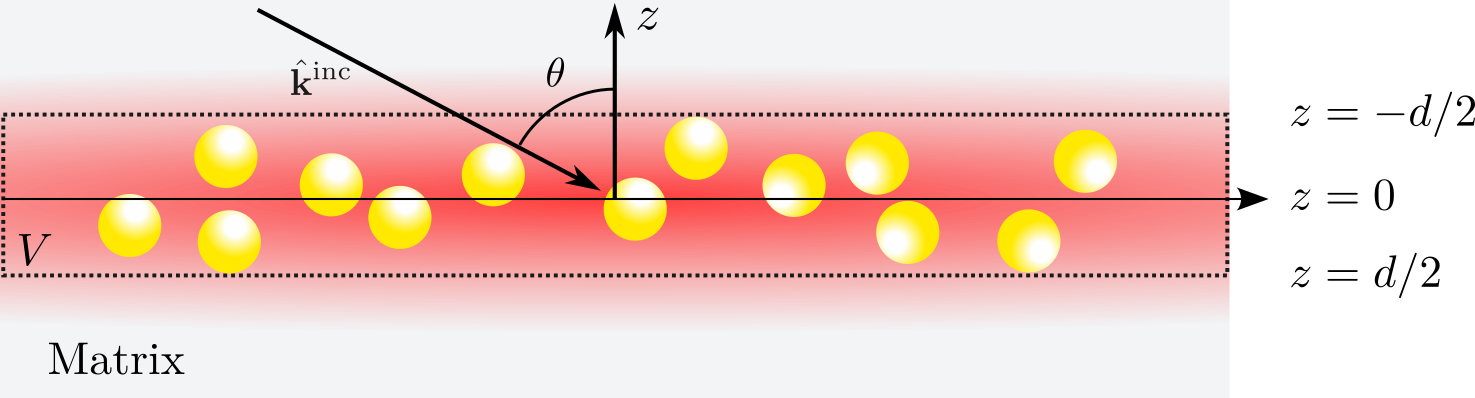
\includegraphics[scale = 1]{img/1-CSM/Fig-CSM.png}
			\end{block}
			\column{.9\squeezetwo}
			
			\begin{align*}
				\vb{E}^\text{exc}_k(\vb{r}) = & 
				\vb{E}^\text{inc}(\vb{r}) + \sum_{\ell\neq k}^N \vb{E}^\text{ind}_\ell(\vb{r})\\
				\vb{E}^\text{ind}_\ell(\vb{r}) = & 
				\int\dd^3 r' \mathbb{G}(\vb{r},\vb{r}') \times
				\int\dd^3 r''\mathbb{T}(\vb{r}'-\vb{r}_\ell,\vb{r}''-\vb{r}_\ell) \vb{E}_\ell^\text{exc}(\vb{r}'')\\
				\textcolor{sblueFC}{\langle\vb{E}(\vb{r})\rangle =} 
				& \textcolor{sblueFC}{\vb{E}^\text{inc}(\vb{r}) +  \sum_{\ell = 1}^N 
					\underbrace{\left(\prod_{k = 1}^N \int\dd^3 r_k \rho(\vb{R}) \vb{E}^\text{ind}_\ell(\vb{r})\right)}_{\text{\normalsize $\langle \vb{E}_\ell^\text{ind}\rangle$}}}
			\end{align*}
			
		\end{columns}
		\vskip1em
		\begin{columns}
			\column{.9\squeezetwo}
			\begin{alertblock}{Aproximación de esparcidor individual (SSA)}
				\begin{align*}
					\langle \vb{E}^\text{ind}_\ell(\vb{r}) \rangle =& \int\dd^3 r'\mathbb{G}(\vb{r},\vb{r}')
					\int\dd^3 r'' \times\\
					& \int \dd^3 r_\ell \rho(\vb{r}_\ell) \mathbb{T}(\vb{r}'-\vb{r}_\ell,\vb{r}''-\vb{r}_\ell)
					\langle \vb{E}_\ell^\text{exc}(\vb{r}'',\vb{R})\rangle_\ell\\
					\langle \vb{E}_\ell^\text{exc}(\vb{r}'',\vb{R})\rangle_\ell
					=& \prod_{\substack{k =1 \\ k\neq \ell}}^N  \int\dd^3 r_k \rho(\vb{R}|\vb{r}_\ell) \vb{E}^\text{exc}_\ell(\vb{r}'')
					\textcolor{sredFC}{ = \vb{E}^\text{inc}(\vb{r}'')}			
				\end{align*}
			\end{alertblock}
			\column{.9\squeezetwo}
			\begin{alertblock}{Aproximación Cuasicristalina (QCA)}
				\begin{align*}
					\langle \vb{E}_\ell^\text{exc}(\vb{r}'',\vb{R})\rangle_\ell =& \vb{E}^\text{inc}(\vb{r}'')
					+ \sum_{\substack{m =1 \\ m\neq \ell}}^N  \int\dd^3 r' \mathbb{G}(\vb{r}',\vb{r}'') \times \notag\\
					& \int\dd^3 r'''\int \dd^3 r_m \rho(\vb{r}_m) \mathbb{T}(\vb{r}'-\vb{r}_m,\vb{r}'''-\vb{r}_m) \langle \vb{E}_m^\text{exc}(\vb{r}'',\vb{R})\rangle_{\ell,m}\\
					\langle \vb{E}_m^\text{exc}(\vb{r}'',\vb{R})\rangle_{\ell,m}
					&= \prod_{\substack{n =1 \\ n\neq \ell,m}}^N  \int\dd^3 r_n \rho(\vb{R}|\vb{r}_\ell,\vb{r}_m) \vb{E}^\text{exc}_n(\vb{r}'')
					\textcolor{sredFC}{ = \langle \vb{E}_\ell^\text{exc}(\vb{r}'',\vb{R})\rangle_\ell}
				\end{align*}
			\end{alertblock}
		\end{columns}	% 
		
		\begin{textblock*}{80mm}(145mm,137.5mm)
			\begin{flushleft}
				\scriptsize
				\rule{30mm}{.5pt}\\
				\footnotemark[1]\fullcite{garcia2012multiple}
			\end{flushleft}
		\end{textblock*}
	\end{frame}
}


\begin{frame}[t]{\underline{Modelo de esparcimiento coherente (CSM)}}
	{Caso monodisperso\footnotemark[1]}
	\centering
	\begin{columns}
		\column{.9\squeezetwo}
		\begin{block}{\centering N esparcidores}
			\centering
			\begin{tasks}(2)
				\task QCA
				\task Esferas de radio $a$
				\task Película de grosor $d\to 0$
				\task $\rho(\vb{r}_\ell) = 1/V$
				\task Correlación de esfera dura
				\task $\alpha = 2\Theta /[(ka)^2 \cos\theta]$
			\end{tasks}
			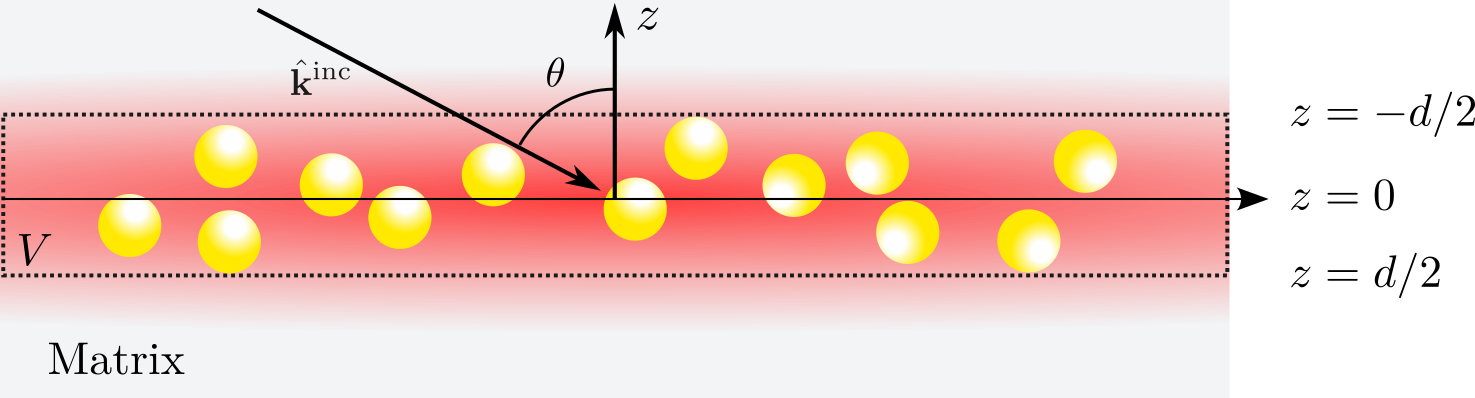
\includegraphics[scale = 1]{img/1-CSM/Fig-CSM.png}
		\end{block}
		\column{\squeezetwo}
		\begin{align*}
			\langle \vb{E}_\text{SSA}^\text{ind}(\vb{r})\rangle &=
			\begin{dcases}
				-\alpha  S_i(\pi-2\theta)	\exp(i\vb{k}^\text{r}_\text{coh}\cdot\vb{r}) \vb{E}^\text{inc}, & z > 0 \\
				-\alpha S(0)\exp(i\vb{k}^\text{t}_\text{coh}\cdot\vb{r}) \vb{E}^\text{inc},  & z < 0 \\
			\end{dcases}
		\end{align*}
		\begin{align*}
			\langle\vb{E}^\text{exc}_\ell(\vb{r}) \rangle_\ell &=
			\vb{E}^\text{exc}_\text{r}(\vb{r})\ \exp(i\vb{k}^\text{r}_\text{coh}\cdot\vb{r}) +
			\vb{E}^\text{exc}_\text{t}(\vb{r})\ \exp(i\vb{k}^\text{t}_\text{coh}\cdot\vb{r})\\
			\langle \vb{E}_\text{QCA}^\text{ind}(\vb{r})\rangle &=
			\begin{dcases}
				-\alpha \bigg( S_j(0) \norm{\vb{E}^\text{exc}_\text{r}(\vb{r})} +  S(\pi-2\theta)\norm{\vb{E}^\text{exc}_\text{t}(\vb{r})}\bigg)
				\exp(i\vb{k}^\text{r}_\text{coh}\cdot\vb{r}) \vu{E}^\text{inc}, & z > 0 \\
				-\alpha \bigg( S_j(\pi-2\theta) \norm{\vb{E}^\text{exc}_\text{r}(\vb{r})} + S(0)\norm{\vb{E}^\text{exc}_\text{t}(\vb{r})}\bigg)
				\exp(i\vb{k}^\text{t}_\text{coh}\cdot\vb{r}) \vu{E}^\text{inc},  & z < 0 \\
			\end{dcases}\\
			\vb{E}^\text{exc}_\text{r}(\vb{r}) &= -\frac{\alpha}{2} \bigg( S_j(0) \norm{\vb{E}^\text{exc}_\text{r}(\vb{r})} +  S(\pi-2\theta)\norm{\vb{E}^\text{exc}_\text{t}(\vb{r})}\bigg) \vu{E}^\text{inc},
			\\
			\vb{E}^\text{exc}_\text{t}(\vb{r}) &= \vb{E}^\text{inc}(\vb{r}) -\frac{\alpha}{2} \bigg( S_j(\pi-2\theta) \norm{\vb{E}^\text{exc}_\text{r}} + S(0)\norm{\vb{E}^\text{exc}_\text{t}(\vb{r})} \bigg)
			\vu{E}^\text{inc}.
		\end{align*}
	\end{columns}
	
	
	\begin{tikzpicture}[node distance=20 mm and 50mm]
		\path (0,0) node [concept]  (meta) {\Large Coeficiente de reflexión y transmisión};
		
		\node[below of=meta] (eqs){
			\begin{minipage}{80mm}
				\begin{align*}
					r^{(j)}_\text{CSM}(\theta)&=\frac{-\alpha S_j(\pi-2\theta)}
					{1+\alpha S(0)+\frac14 \alpha^2 \left[S^2(0)-S_j^2 (\pi-2\theta) \right]}\\
					t^{(j)}_\text{CSM}(\theta)&=\frac{1-\frac14\alpha^2\qty[S^2(0)-S_j^2(\pi-2\theta)]}
					{1+\alpha S(0)+\frac14 \alpha^2 \left[S^2(0)-S_j^2 (\pi-2\theta) \right]}
				\end{align*}
		\end{minipage} };
		
		\node [flowbox, right=of eqs] (sus) {\fbtitle{Presencia de sustrato (Reflexión)}
			\nodepart{two}
			\begin{minipage}{80mm}
				\begin{align*}
					r^{(j)}(\theta_i)&= \frac{r_\text{sm}^{(j)}(\theta_i) + r_\text{CSM}^{(j)}(\theta_t)}
					{1+r_\text{sm}^{(j)}(\theta_i) r_\text{CSM}^{(j)}(\theta_t)}
				\end{align*}
		\end{minipage}};
		
		\draw[hidden] (eqs.east) -- 
		node[above,text=sdgrayFC,font=\itshape\scriptsize,anchor=south] {Múltiples reflexiones}
		(sus.west);
	\end{tikzpicture}
	
	\begin{textblock*}{80mm}(145mm,137.5mm)
		\begin{flushleft}
			\scriptsize
			\rule{30mm}{.5pt}\\
			\footnotemark[1]\fullcite{garcia2012multiple}
		\end{flushleft}
	\end{textblock*}
	
\end{frame}


\begin{frame}[c]{\underline{Teoría de película delgada (TFT)}}
	{Condiciones de frontera modificadas\footnotemark[1]}
	\centering
	\begin{tikzpicture}[node distance=10 mm and 15mm]
		\path (0,0) node [concept]  (meta) {\large Ecuaciones de Maxwell para campos de exceso};
		
		\node[below right =of meta,xshift=-15mm ] (PM) {%
			\begin{minipage}{50mm}
				\begin{align*}
					\vb{P}^\text{film}(\vb{r}_\parallel) &= \vb{D}_\parallel^\text{film}(\vb{r}_\parallel) - \varepsilon_0 {E}_\perp^\text{film}(\vb{r}_\parallel) \vu{e}_\perp\\
					%	
					\vb{M}^\text{film}(\vb{r}_\parallel) &= \frac{1}{\mu_0}\vb{B}_\parallel^\text{film}(\vb{r}_\parallel) -  {H}_\perp^\text{film}(\vb{r}_\parallel) \vu{e}_\perp
				\end{align*}
		\end{minipage}};
		
		\node [flowbox, fb-highlight, below right =of PM] (cf) {\fbtitle{Condiciones de frontera}
			\nodepart{two}
			\begin{minipage}{50mm}
				\begin{align*}
					\qty[D_\perp^>(\vb{r}_\parallel)-D_\perp^<(\vb{r}_\parallel)]  & = -\nabla_\parallel\cdot\vb{P}_\parallel^\text{film}(\vb{r}_\parallel)\\
					%	
					\qty[B_\perp^>(\vb{r}_\parallel)-B_\perp^<(\vb{r}_\parallel)]  & = -\nabla_\parallel\cdot\vb{M}_\parallel^\text{film}(\vb{r}_\parallel)\\
					%	
					\qty[\vb{E}^>_\parallel(\vb{r}_\parallel)-\vb{E}^<_\parallel(\vb{r}_\parallel)] & = -i{\omega}\vu{e}_\perp\times \vb{M}^\text{film}_\parallel(\vb{r}_\parallel)-\nabla_\parallel P_\perp^\text{film}(\vb{r}_\parallel)\\
					%	
					\qty[\vb{H}^>_\parallel(\vb{r}_\parallel)-\vb{H}^<_\parallel(\vb{r}_\parallel)] & = +i{\omega}\vu{e}_\perp\times \vb{P}^\text{film}_\parallel(\vb{r}_\parallel)-\nabla_\parallel M_\perp^\text{film}(\vb{r}_\parallel)
				\end{align*}
		\end{minipage}};
		
		\node[concept, above=of cf, yshift=30mm] (const) {Ecuaciones constitutivas};
		\node[below =of const, yshift=15mm] (const-eq) {\begin{minipage}{50mm}
				\begin{align*}
					\vb{P}^\text{film}(\vb{r}_\parallel) &= 
					\gamma\,\big\langle\vb{E}^\text{film}_\parallel(\vb{r}_\parallel)\big\rangle +
					\beta \,\big\langle {D}^\text{film}_\perp(\vb{r}_\parallel)\big\rangle \vu{e}_\perp\\
					\vb{M}^\text{film}(\vb{r}_\parallel) &= \vb{0}
				\end{align*}
		\end{minipage}};
		
		\draw[hidden] (meta.south) |-
		node[above,text=sdgrayFC,font=\small,anchor=east]
		{\begin{minipage}{30mm}
				\begin{flushright}
					Límite de película delgada\\
					Transformada de Fourier en $z$\\
					$k_z = 0$
				\end{flushright}
		\end{minipage}}
		(PM.west);
		%	$\big\langle a^\text{film} (\vb{r}_\parallel)\big\rangle~=~(1/2)[a^>(\vb{r}_\parallel) + a^<(\vb{r}_\parallel)]$
		\draw[hidden] (PM.315) |- (cf.west);
		\draw[hidden] (PM.45) |- node[below, near end,text=sdgrayFC,font=\small,anchor=south]
		{$\big\langle a^\text{film} (\vb{r}_\parallel)\big\rangle~=~(1/2)[a^>(\vb{r}_\parallel) + a^<(\vb{r}_\parallel)]$}
		(const.west);
		\draw[hidden] (const-eq.south) -- (cf.north);
		
		
		\node[below =of meta, yshift=-50mm] (diagrama) {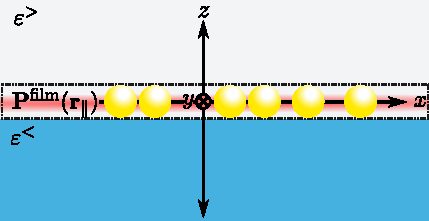
\includegraphics[scale=1]{img/2-TFT/monolayer.pdf}};
		\node[right=of diagrama, xshift=-18mm] {\begin{minipage}{60mm}
				\begin{itemize}
					\item $\gamma = \dfrac23 \dfrac{\Theta}{V_\text{sp}} \qty( \dfrac{\alpha_\text{sp}}{1 + A \alpha_\text{sp}})$
					\item $\beta =\dfrac23 \dfrac{\Theta}{\varepsilon_i^2 V_\text{sp}} \qty(\dfrac{\alpha_\text{sp}}{1 + 2 A \alpha_\text{sp}})$
					\item $\alpha_\text{sp} = 3  \varepsilon_t V_\text{sp} \qty(\dfrac{\varepsilon_\text{sp} - \varepsilon_t}{\varepsilon_\text{sp} + 2 \varepsilon_t})$
					\item $A = \dfrac{\varepsilon_i - \varepsilon_t}{\varepsilon_i + \varepsilon_t}$
				\end{itemize}
		\end{minipage}};
	\end{tikzpicture}
\end{frame}




\begin{frame}{Ajuste de parámetros}
	{\textoverline{Minimización del error mediante descenso de gradiente}}
	
	\begin{center}
		\begin{tikzpicture}[node distance=15mm and 40mm]
			\setlength{\leftmargini}{10pt}
			
			% mono
			\path (0,1.25) node[concept,align=center] (modelo) {
				Modelo teórico
			};
			\node[below=of modelo,yshift=15mm] {%
				\begin{minipage}{1.5cm}
					$\begin{aligned}
						&\vec{x} \equiv \text{Parámetros}\\
						&f_i(\vec{x}) \equiv \text{Modelo}\\
					\end{aligned}$
				\end{minipage}
			};
			
			\path (0,-5) node[concept,align=center] (exp) {
				Resultado experimental
			};
			\node[below=of exp,yshift=15mm] {%
				\begin{minipage}{1.5cm}
					$\begin{aligned}
						y_i(\vec{x}) &\equiv \text{Medición}\\
					\end{aligned}$
				\end{minipage}
			};
			
			\node[below right = of modelo, concept,align=center,yshift=-.5cm] (error) {
				Error};
			
			\node[below =of error,yshift=15mm](min){
				$\begin{aligned}
					F(\vec{x}) = \frac{1}{N}\sum_{i=1}^N\qty(f_i(\vec{x})-y_i)^2
				\end{aligned}$
			};
			
			\draw[hidden] (modelo.east) -| (error.north) ;
			\draw[hidden] (exp.east) -| (min.south) ;
			
			\node[flowbox,fb-highlight,right =of error,xshift=0cm] (des) {%
				\fbtitle{Descenso de gradiente}\vphantom{yÖ}
				\nodepart{two}
				\begin{minipage}{35mm}\centering
					\begin{align*}
						\vec{x}_{\ell+1} = \vec{x}_\ell - \gamma \nabla F(\vec{x}_\ell)
					\end{align*}
				\end{minipage}
			};
			
			\draw[hidden] (error.east) -- (des)
			node[right,near start,text=sdgrayFC,font=\itshape\small,anchor=south] {
				Minimización
			};
			
			\node[flowbox,below=of des,yshift=-2cm] (barzilai) {%
				\fbtitle{Método de dos pasos}\vphantom{yÖ}
				\nodepart{two}
				\begin{minipage}{60mm}
					\begin{align*}
						\gamma_\ell = \frac{\qty(\vec{x}_{\ell} - \vec{x}_{\ell-1}) \cdot  \qty[\nabla F(\vec{x}_\ell)-\nabla F(\vec{x}_{\ell-1})]}
						{\norm{\nabla F(\vec{x}_\ell)-\nabla F(\vec{x}_{\ell-1})}^2}
					\end{align*}
				\end{minipage}
			};
			
			\draw[conn] (des) -- (barzilai);
		\end{tikzpicture}
	\end{center}
	
	
\begin{textblock*}{80mm}(145mm,137.5mm)
		\begin{flushright}
			\scriptsize
		   \fullcite{barzilai_two-point_1988}
		\end{flushright}
	\end{textblock*}
	
\end{frame}


\begin{frame}{Metasuperficie vs. partícula individual}
	{\textoverline{Longitudes de onda de excitación de una metasuperficie plasmónica en ATR}}
	\centering
			\begin{tabular}{c|c||cc||c|c} \hline\hline
		&   & \multirow{2}{8em}{Radio considerado {[}nm{]}} & \multirow{2}{11em}{\centering Fracción de cubierta considerada $\Theta$} & \multicolumn{2}{c}{Longitud de onda de excitación [nm]} \\ 
		&   & &    & $\theta_i = 64.9^\circ$  & $\theta_i = 72.9^\circ$ \\  \hline\hline
		\multirow{8}{*}{\rotatebox{90}{Polarización $s$}}& \multirow{2}{*}{Experimental}   & 5.78  & 0.20  & 536.71  & 552.36 \\
		&									& 7.30	& 0.22  & 536.07  & 569.53\\ \cline{2-6}
		& \multirow{2}{*}{CSM (Valores nominales)}						& 5.78  & 0.20  & 525.05  & 531.53 \\
		&									& 7.30	& 0.22  & 525.05  & 534.77 \\ \cline{2-6}
		& \multirow{2}{*}{CSM (Fit @ $64.9^\circ$)} 				& 3.56  & 0.25  & 525.05  & -  \\
		&								    & 5.29  & 0.27  & 525.05  & -  \\ \cline{2-6}
		& \multirow{2}{*}{CSM (Fit @ $72.9^\circ$)}					& 3.45  & 0.25  & - & 531.53    \\
		&   								& 5.45  & 0.27  & - & 534.77 \\ \hline\hline
		\multirow{8}{*}{\rotatebox{90}{Polarización $p$}} & \multirow{2}{*}{Experimental}   & 5.78  & 0.20   & 513.44 & 525.69 \\
		&								    & 7.30	& 0.22  & 511.68  & 522.89 \\ \cline{2-6}
		& \multirow{2}{*}{CSM (Valores nominales)} 					& 5.78  & 0.2   & 525.05  & 534.77 \\
		&							   	 	& 7.30	& 0.22  & 525.05  & 538.06 \\ \cline{2-6}
		& \multirow{2}{*}{CSM (Fit @ $64.9^\circ$)} 				& 3.29  & 0.17  & 525.05  & -  \\
		&								    & 4.03  & 0.19  & 525.05  & -  \\ \cline{2-6}
		& \multirow{2}{*}{CSM (Fit @ $72.9^\circ$)}					& 3.34  & 0.17  & - & 531.53 \\
		&								    & 4.11  & 0.19  & - & 534.77 \\ \hline\hline
	\end{tabular}
	
\end{frame}